\section{Clusters: conservative dynamics and observed targets}
\label{sec:clusters}

The cluster calculation uses positive, inertial stock, gas, and stars in
one gravitational potential. Gas pressure and shocks can separate the
gas from the weakly coupled stock and galaxies during an encounter.
The observed lensing map measures their total projected mass. This
construction supplies a transport mechanism and quantitative targets;
the present comparisons do not constitute a fitted cluster population.
\source{CL1--CL3}

\subsection{A common mass budget and a conservative encounter}
For a fully released closed cohort, the adopted normalization in the
formation mass convention of the cosmological fit is
\begin{equation}
k_C=5.333\,e^{-\eta_*}=5.1760752,\qquad C_0=k_C B_0.
\end{equation}
The bare convention gives $e^{-\eta_*}/\epsilon=5.164$.
If its baryons and stock remain coextensive, the baryon fraction is
$1/(1+k_C)=0.1619151$. More generally, an aperture retains different
fractions of the ancestral components. The measured target can be
expressed as
\begin{equation}
C_{\rm req}=M_{\rm grav}-B,\qquad
\eta_{\rm ret}=\frac{k_C B}{C_{\rm req}}
=\frac{f_b^{\rm ret}}{f_C^{\rm ret}}.
\end{equation}
This distinguishes the common cohort normalization from the distribution
produced by assembly. A positive inventory exists for $C_{\rm req}>0$:
$B_0=\max(B,C_{\rm req}/k_C)$ leaves nonnegative exterior baryons
$B_0-B$ and stock $k_CB_0-C_{\rm req}$. It does not determine a
realizable transport history or its energy cost.

The encounter model uses central pair impulses with opposite momentum
changes. If $w$ is the radial relative velocity and $\mu$ the reduced
mass, the kinetic change is $\Delta K=\mu(w'^2-w^2)/2$. Explicit work
and heat registers balance that change, and a symmetric gate suppresses
transitions with an endpoint at the energy floor. Gas and stars from
either progenitor can be local partners. The target distribution, rate,
range, and initial work reserves are selected effective inputs.
\source{D2, CL1}

Fourteen encounters and three isolated controls test a common Plummer
mass ratio of 0.3, with 1344 particles at baseline and 2688 in the
resolution control. Weak contact leaves stock near the galaxies while
gas lags. A floor-state run permits no events and reproduces the
no-contact evolution; a low-work run permits 61 events against 7114
with the larger reserve. The largest energy drift is below 0.007\%
of the binding energy; pair momentum conservation holds at roundoff.
The strongest tested contact changes the isolated stock median radius
by $-27\%$ and gas median radius by $+46\%$ in six dynamical time units.
That control prevents interpreting a higher contact rate as an established
cluster solution. The particle encounters test the finite-work coupling;
they do not evolve the full spatial stress of the depleted scalar.

\subsection{X-COP profiles and independent weak-lensing masses}
The public X-COP archive supplies twelve hydrostatic radial profiles,
seven with stellar mass data. Five overlap the MENeaCS lensing catalogue.
The comparison adopts the observational distance convention
$H_0=70\,\kms\,\mathrm{Mpc}^{-1}$ and $\Omega_m=0.3$.
Projected stellar masses are approximately deprojected using the stated
profile model. Unmeasured intracluster light, hydrostatic departures,
triaxiality, and profile covariance remain relevant.
\cite{xcopnew,herbonnetnew}\source{CL2}

All nominal NFW hydrostatic targets admit positive cumulative stock and
positive stock in fifteen tested shells. At the hydrostatic $R_{500}$,
the coextensive-to-hydrostatic total-mass ratios for A1795, A2029, A2142,
A2319, A644, A85, and ZW1215 are respectively
$0.903$, $0.912$, $1.023$, $1.213$, $0.851$, $0.952$, and $0.679$.
These reconstructed totals are inputs to a target audit, rather than
stock profiles predicted from the observed baryons.

\begin{table}[H]
\centering\small
\begin{tabular}{lrrr}
\toprule
Cluster & Coextensive $M_{500}$ & Lensing $M_{500}$ & $\eta_{\rm ret}$\\
\midrule
A1795 & 3.96--4.23 & $9.3\pm2.2$ & 0.518\\
A2029 & 7.46--8.07 & $12.1\pm2.5$ & 0.704\\
A2142 & 9.29--10.02 & $9.7\pm2.3$ & 0.969\\
A85 & 5.20--5.43 & $5.7\pm2.2$ & 0.937\\
ZW1215 & 4.19--4.46 & $3.5\pm2.2$ & 1.143\\
\bottomrule
\end{tabular}
\caption{Masses in $10^{14}\Msun$. The coextensive prescription solves
its own overdensity radius; its range doubles the nominal stellar mass
and is a sensitivity interval. Retention ratios use the nominal baryons
within each central lensing target's radius. Lensing errors are the
published NFW marginal errors. No combined exclusion significance is
assigned.}
\end{table}

\begin{figure}[H]
\centering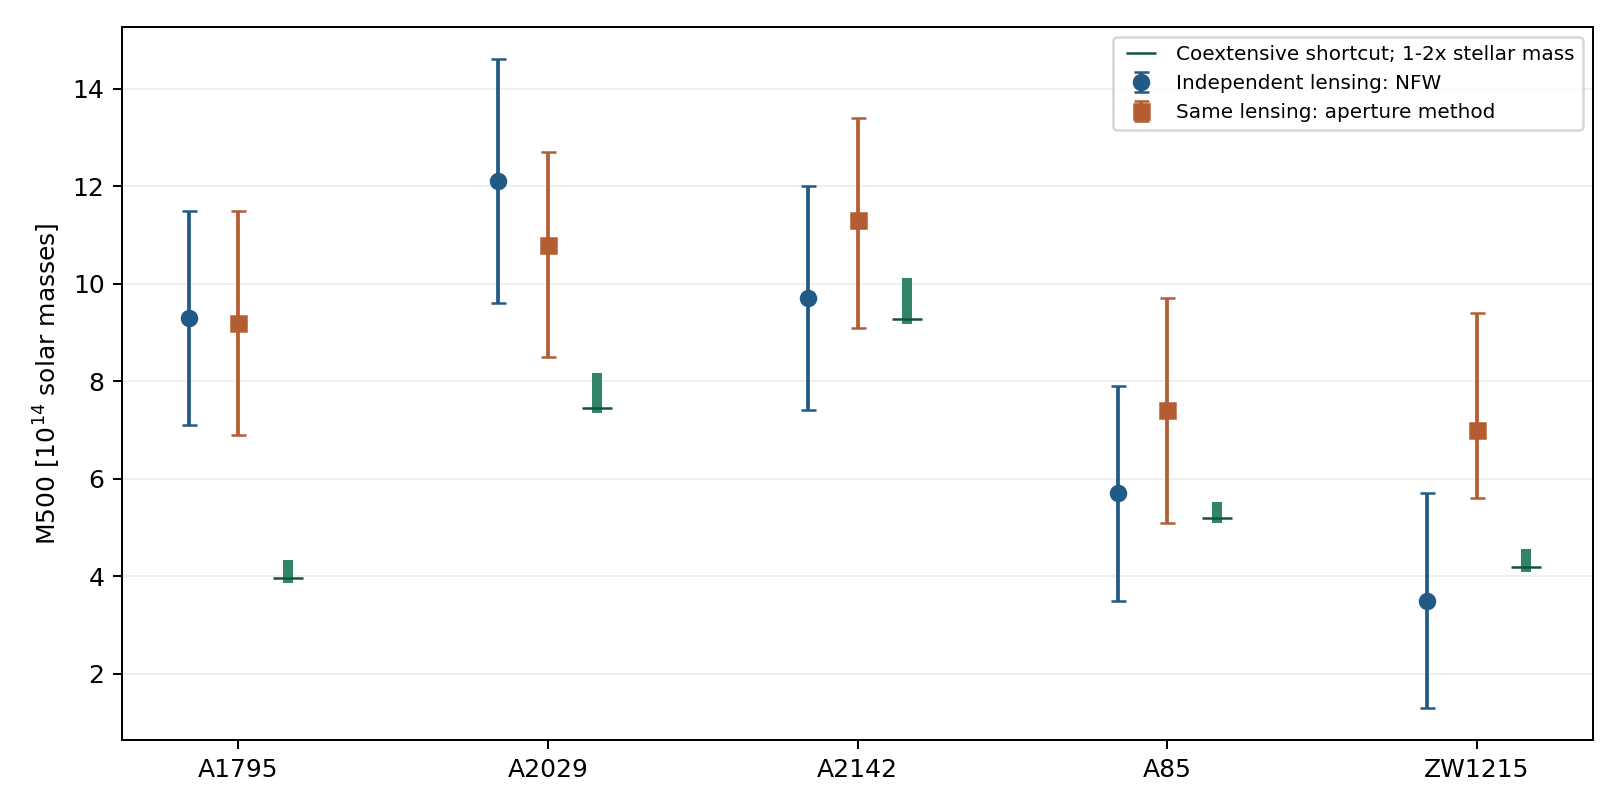
\includegraphics[width=\textwidth]{figures/cluster_lensing.png}
\caption{The common coextensive prescription and two mass estimators
from the same lensing data. Their errors are correlated. A1795 and
A2029 require a transport or reconstruction explanation; A2142 and A85
are useful normalization controls. ZW1215 is sensitive to the estimator.}
\end{figure}

\subsection{Why clusters remain fair samples}
The stock that reaches the galactic response law in isolated galaxies
(Section~\ref{sec:stockselection}) is the same stock that fills clusters.
The selection acts through the cells of active carriers, on the stock each
carrier carries. A carrier's records are identified with its condensed
baryons, stars and cold gas; virialized hot gas relaxes toward the Gibbs state
of its potential. A carrier's support ends where its records stop dominating
the enclosed baryons, and its cells act on the stock bound to the potential of
its records and the stock it carries.
In the X-COP clusters the supports and cell energies are:
\begin{center}
\small
\begin{tabular}{lcccc}
\toprule
Cluster & $r_d$ (kpc) & $r_d/R_{500}$ & condensed fraction at $R_{500}$ & cell energy ((km/s)$^2$)\\
\midrule
A85 & 47 & 0.038 & 0.025 & 21\\
A1795 & 65 & 0.056 & 0.044 & 90\\
A2029 & 76 & 0.054 & 0.052 & 93\\
A2142 & 68 & 0.048 & 0.047 & 37\\
A2319 & 99 & 0.072 & 0.035 & 121\\
A644 & 87 & 0.069 & 0.051 & 132\\
ZW1215 & 97 & 0.071 & 0.038 & 55\\
\bottomrule
\end{tabular}
\end{center}
Here $r_d$ is the radius where projected stellar mass equals gas mass, an upper
bound, and the cell energy is per unit cluster stock. Outside $r_d$, and for
stock crossing it unbound, the cluster stock is collisionless and keeps the
cohort ratio of the common mass budget. The X-COP medians test that ratio:
\begin{center}
\begin{tabular}{lcc}
\toprule
& total/baryon & source\\
\midrule
Cohort prediction $1+k_C$ & 6.18 & theory\\
X-COP median, $R_{500}$ & 6.45 & hydrostatic, $f_\star=0.015$\\
X-COP median, $R_{200}$ & 6.10 & hydrostatic, $f_\star=0.015$\\
Response law at $R_{500}$ ($g_{\rm bar}=0.05$--$0.07\,a_0$) & 4.2--5.0 & theory\\
Cohort stock plus an always-on response & 9.4--10.2 & theory\\
\bottomrule
\end{tabular}
\end{center}
A response acting on cluster stock fails in either direction. Galaxy
outskirts that obey the law lie at the same $g_{\rm bar}/a_0$, at 35--50\,kpc in
a Milky Way model, so the switch cannot depend on acceleration alone.

Contact runs start from the observed profiles of the seven clusters with the
archived contact kernel, conservative softened gravity and fixed baryons, and
compare with matched no-contact controls after 8--10\,Gyr, at three contact
proposals per orbit:
\begin{center}
\small
\begin{tabular}{lccc}
\toprule
Rule & $R_{500}$ & $0.3R_{500}$ & $0.1R_{500}$\\
\midrule
Cells throughout, galactic work allowance & 0.547--0.787 & 0.319--0.440 & 0.209--0.366\\
Support only, galactic work allowance & 0.976--0.997 & 0.867--0.961 & 0.369--0.731\\
Support only, cell work & 0.997--1.007 & 0.990--1.019 & 0.563--0.937\\
Support, carried stock, cell work & 0.9998--1.0008 & 0.997--1.002 & 0.985--1.007\\
\bottomrule
\end{tabular}
\end{center}
\begin{figure}[H]
\centering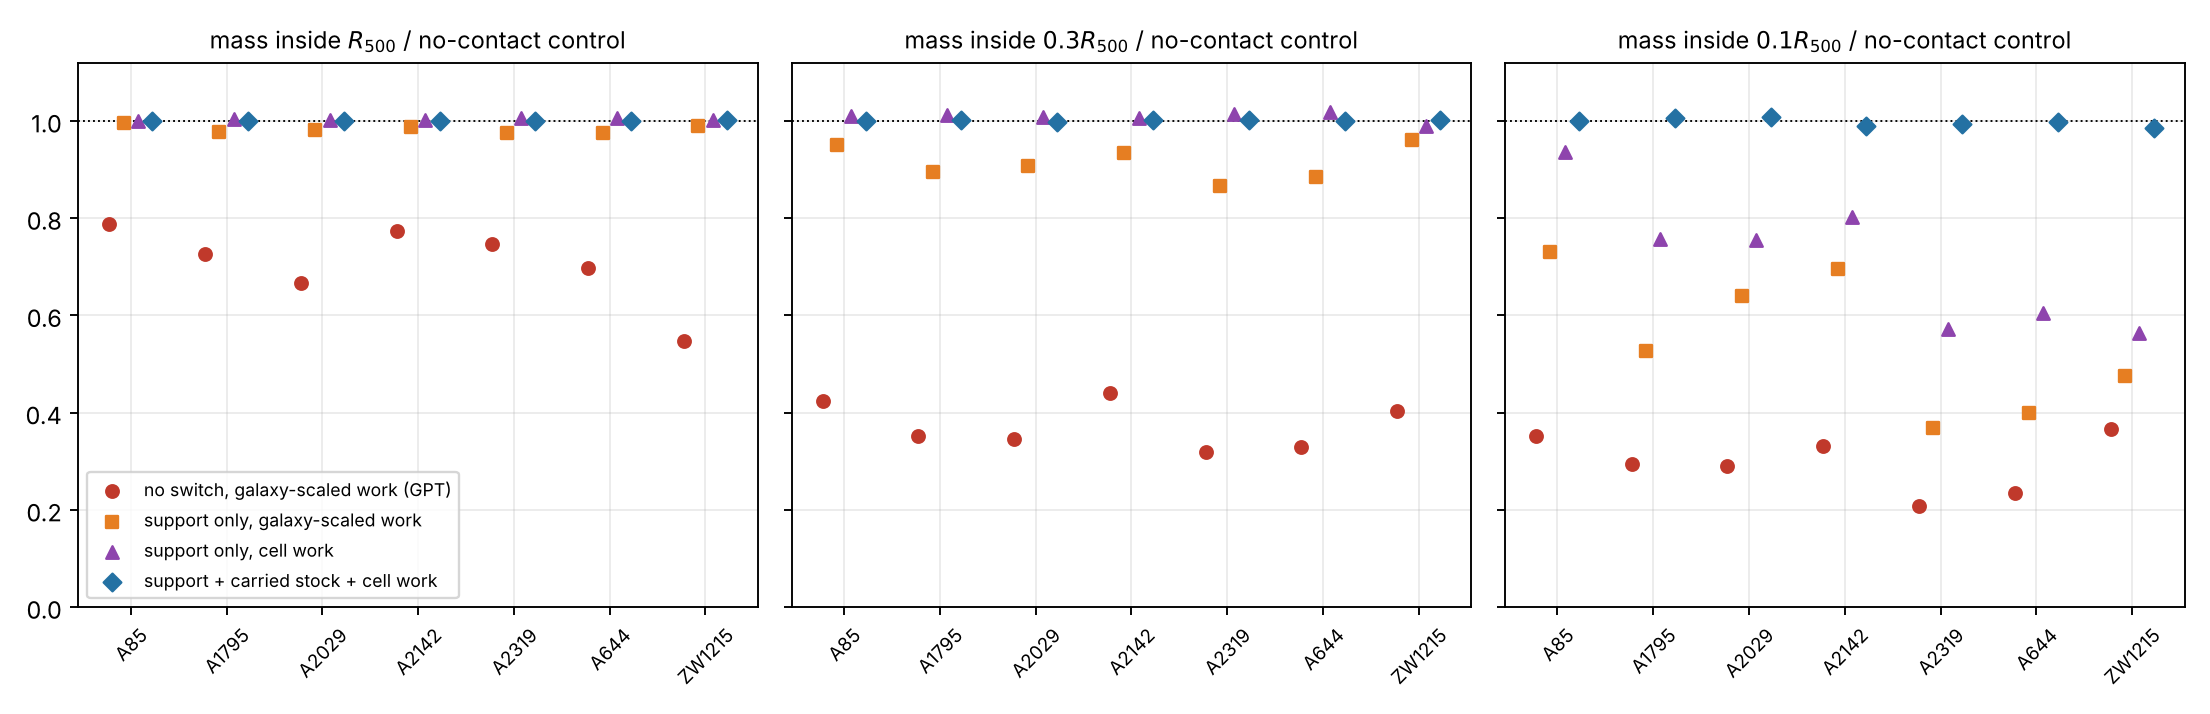
\includegraphics[width=\textwidth]{figures/cluster_switch.png}
\caption{Mass inside three radii relative to the no-contact control for the
four rules of the table, with 2000, 2000, $10^4$ and $1.6\times10^4$
particles.}
\end{figure}
Contacts are confined to 4--7\% of $R_{500}$ with $10^{-4}$ of the binding
energy, so the outer result follows from the support. With support only, the
central galaxy's cells drain the uncarried cluster stock in its support to
7--30\% of the control. With carried stock, averaged over 8--10\,Gyr, the core
keeps 94--105\% inside $r_d$ and 99--101\% inside $2r_d$, with a Poisson error
of 6--14\%. The central galaxy's carried stock falls from 1.1--4.3 to
0.57--0.85 times its galactic-law value, and its support keeps 7--11 times
that value in uncarried stock. The same rule leaves isolated galaxies on the
law inside their supports, which for the Milky Way end at 115--490\,kpc.
The X-ray ellipticals on the radial acceleration relation \cite{lelli17}
test the record identification directly. Over the radii used there, stars
dominate their enclosed baryons; in NGC~720 hot gas becomes the dominant
baryonic component only outside about 200\,kpc \cite{humphrey11}. Excluding
the hot gas from the record source lowers the outermost points by at most
0.04\,dex. Isolated ellipticals hold no group stock and should follow the law
out to the radius where their hot gas dominates. Carrier support
makes four observational distinctions:
\begin{itemize}
\item central galaxies of groups and brightest cluster galaxies depart
from the rotating-galaxy relation, with an acceleration scale about
17 times larger for brightest cluster galaxies \cite{bcgrar,centralsrar};
\item X-ray groups at 0.5--2\,keV require mass beyond the response law
\cite{angus08}, as retained collisionless stock supplies;
\item in X-ray groups the excess over the law begins in the core: in A262,
MKW4 and RXJ1159.8+5531 it exceeds 0.1\,dex within 5--13\,kpc, while hot gas
overtakes the condensed baryons only at 85--210\,kpc
\cite{gastaldello07,vikhlinin06}, so the excess traces the uncarried group
stock;
\item isolated ellipticals follow the law out to the radius where their hot
gas outweighs their stars; NGC~720 lies within about 0.1\,dex of it at
102\,kpc in mass models extrapolated beyond the X-ray data \cite{humphrey11}.
\end{itemize}
Resolved member galaxies and cosmological assembly are the open parts.
\source{G8, G9, G10, G11}

\subsection{What the outliers require}
The central A1795 and A2029 lensing targets require respectively
48.2\% and 29.6\% of the minimal cohort's initial baryons outside the
aperture; for A1795 this is $7.87\times10^{13}\Msun$. Twelve finite
transport maps preserve positive marginals for the seven hydrostatic
and five lensing targets. This inventory construction leaves the
assembly time and work requirement undetermined. \source{CL3}

The gas must obey the same total potential,
\begin{equation}
a_g=-g-\frac{P_{\rm th}'+P_{\rm nt}'}{\rho_g}+\frac{f_{Cg}}{\rho_g}.
\end{equation}
Segregation, acceleration, and reciprocal contact are possible contributions.
Passive drag vanishes at zero drift, so stationary contact support requires
its own physical law. XRISM's low turbulent support in A1795 and A2029
constrains a purely turbulent explanation. \cite{sarkarnew,xrismnew}
The conditional pressure audit also depends on inner lensing extrapolation
and thermal reconstruction; a joint fit remains open.

A644's 58-knot forward profile contains 11 negative total-mass increments
and 15 negative stock increments. A monotone reconstruction requires
2.156 marginal error units of maximum displacement; absent joint
covariance, this is not an exclusion significance. Positive parametric
profiles require comparison with the underlying gas data. For ZW1215,
at 1320 kpc the correlated NFW-lensing, aperture-lensing, and hydrostatic
estimates are $4.32$, $7.0$, and $7.41\times10^{14}\Msun$. Both systems
retain reconstruction uncertainty rather than a new gravity coefficient.

\subsection{The Bullet Cluster supplies a spatial target}
The CANUCS Bullet v1 best-fit maps separate a total lens reconstruction
from a supplied gas component. At lens redshift 0.296 and
$D_{ls}/D_s=1$, their normalization gives
$\Sigma_{\rm crit}=1.8268761\times10^9\Msun\,\mathrm{kpc}^{-2}$
and $1''=4.41302$ kpc. Registered apertures around BCG3 give
\begin{center}
\begin{tabular}{lrrr}
\toprule
Radius & $M_{\rm total}/10^{13}\Msun$ & $M_g/10^{13}\Msun$ & Gas fraction\\
\midrule
60 kpc & 2.151 & 0.099 & 0.046\\
150 kpc & 8.511 & 0.618 & 0.073\\
\bottomrule
\end{tabular}
\end{center}
The released subcluster halo centre lies 3.92 kpc from BCG3. The
supplied gas-density map peaks about 169 kpc away within the specified
search region, with an 8.68 kpc gas pixel. This is a density-map
diagnostic, rather than an X-ray brightness peak or an offset posterior.
Subtracting gas leaves a component that still includes stars.
\cite{bulletnew}\source{CL2}

\begin{figure}[H]
\centering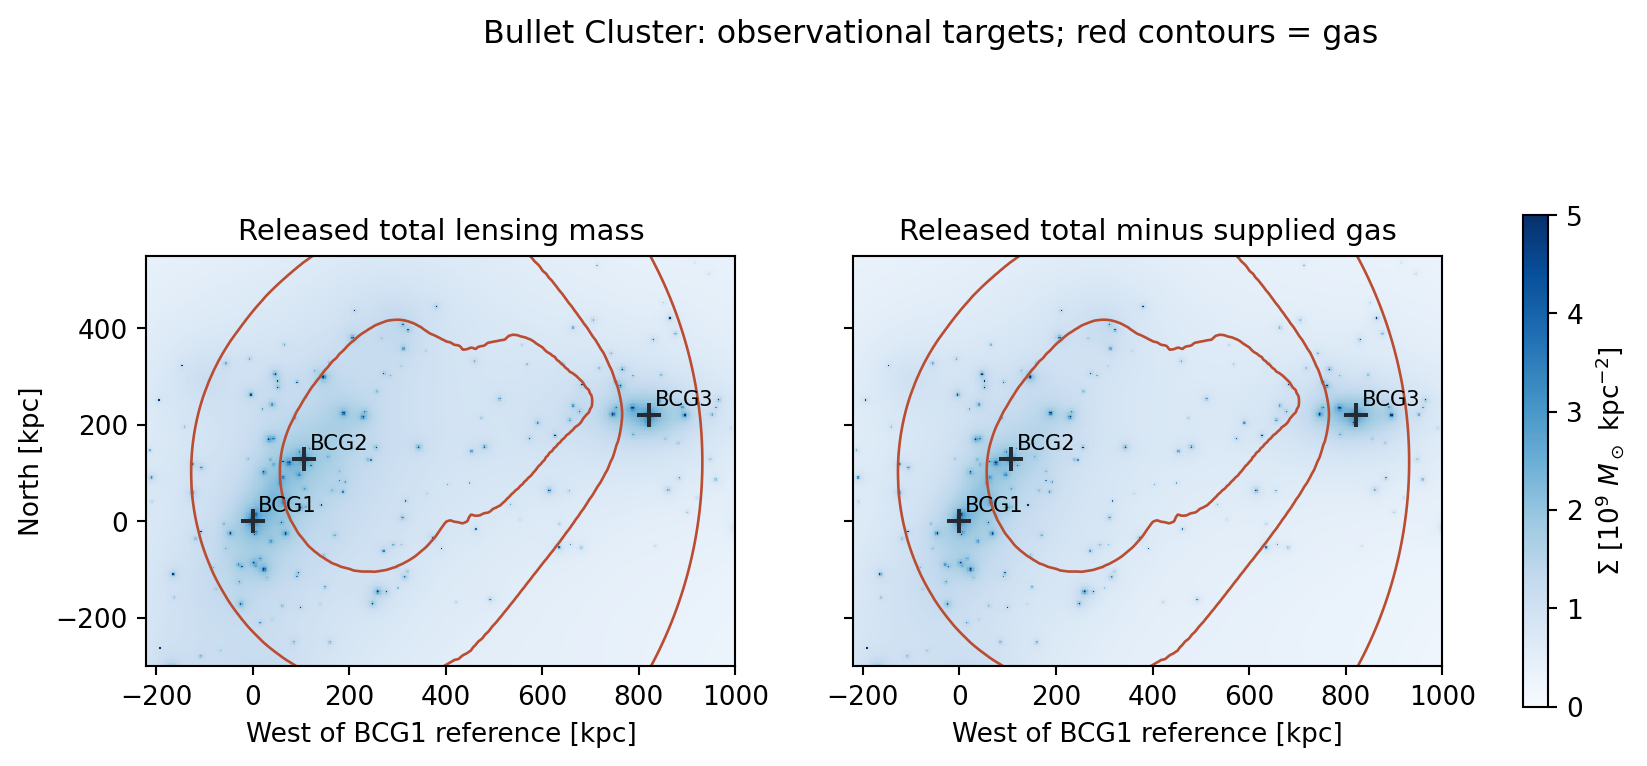
\includegraphics[width=\textwidth]{figures/cluster_bullet.png}
\caption{Observed targets from the released Bullet v1 lens model.
The red contours show its supplied gas component. Both panels are
derived from the public reconstruction; no simulated map is fitted here.}
\end{figure}

Aperture masses change by at most 0.214\% under pixel coarsening; this
is a numerical check and excludes observational uncertainty. Under an
illustrative $10^{15}\Msun$, 300 kpc scaling, the encounter calculations
have 24--30 kpc force softening and roughly 90 kpc map smoothing. They
cannot establish agreement with the few-kiloparsec halo--galaxy alignment.
A successful forward test must preserve isolated cluster profiles and
then reproduce lensing, gas morphology, and offsets using one selected
contact law and independently specified assembly conditions.

